\addchap{Die Fakultät Informatik}

Der \emph{Andreas-Pfitzmann-Bau} (kurz APB) beherbergt die Fakultät Informatik und wird damit in den nächsten Jahren dein zweites Zuhause sein.
Mit zunehmender Semesterzahl wirst du immer weniger über den Campus gescheucht und immer mehr Veranstaltungen werden hier stattfinden.
Doch was hat dieser Bau eigentlich zu bieten außer einer Menge grüner Farbe und der Skulptur im Foyer?

\begin{figure}[h!]
    \centering
    \includegraphics[width=\linewidth]{img/panorama_fakultaet.jpg}
    \caption*{\small \textit{Der Andreas-Pfitzmann-Bau von vorne -- Foto: Lucas Vogel}}
\end{figure}

Ein Unterschied zwischen diesem Gebäude und den anderen auf dem Campus ist, dass es rund um die Uhr geöffnet ist. Auch wenn nachts mal die Türen verschlossen sein sollten, wird dir der Sicherheitsdienst gerne gegen Vorlage deines Studentenausweises die Tür öffnen und auf Wunsch auch einen der Seminarräume im Erdgeschoss aufschließen.

Sitzgelegenheiten auf den Gängen aller Etagen bieten dir genügend Platz, um dich beispielsweise mit deinen Lerngruppen auf anstehende Prüfungen vorzubereiten. Weiterhin gibt es mehrere zum Teil mit Spezial-Software ausgestattete PC-Pools, die jedoch nur tagsüber geöffnet sind.

Außerdem können wir einen ziemlich schicken Außenbereich unser Eigen nennen. Dazu gehört ein Teich und viel Platz auf der Wiese zum Rumlümmeln. Dafür haben wir Decken zur Verfügung gestellt, die nur darauf warten, genutzt zu werden.

\begin{figure}[t]
    \centering
    \includegraphics[width=\linewidth]{img/panorama_teich.jpg}
    \caption*{\small \textit{Der Andreas-Pfitzmann-Bau hinten raus -- Foto: Lucas Vogel}}
\end{figure}

Mit dieser Idylle könnte es jedoch schon bald vorbei sein, da der Außenbereich einem neuen Gebäude weichen soll. Neben vielen Angehörigen der Fakultät hielten auch deine Studierendenvertreter dagegen und machten mit der Aktion \#SaveTheTeich auf das Vorhaben aufmerksam~\link{https://savethetei.ch/}.
Das große Engagement und die zähen Verhandlungen haben sich gelohnt: Der Teich soll nach Ende des Baus größtenteils wiederhergestellt werden. Zur Kompensation der verloren gegangenen Plätze am aktuellen Hang wurden nun überdurchschnittlich viele Mittel für die Ausstattung der übrigen Flächen mit Sitzgelegenheiten und ausreichend Grün vorgesehen.

Vom Teich aus kannst du das Rechenzentrum (\enquote{Lehmann-Zentrum}) sehen. Vielleicht bekommst du ja die Chance, an einer der Führungen durch das Rechenzentrum teilzunehmen, die zu verschiedenen Events angeboten werden.

Seinen Namen entleiht das Gebäude übrigens von Andreas Pfitzmann, einem 2010 verstorbenen Professor aus unserem Hause.
Er leitete über viele Jahre die Professur für Datenschutz und Datensicherheit, an welcher er maßgeblich an Möglichkeiten zur Anonymisierung forschte und so vielen Menschen in Ländern mit Zensur und staatlicher Überwachung freien Internetzugang ermöglichte. Im Jahr 2009 wurde er außerdem Dekan unserer Fakultät.
Im Foyer findest du eine Tafel, welche ihm und seinem Lebenswerk gedenkt.

\pagebreak

\minisec{\textbf{ascii} – Das Café in der Fakultät}

Bereits seit 2007 existiert im Gebäude der Fakultät Informatik das \ascii{}, ein Café betrieben von Studierenden, die ein paar Stündchen ihrer Freizeit zur Verfügung stellen, um hinter dem Tresen zu stehen.

Das \ascii{} hat alles was ein richtiges Café so braucht: Kaffee, Tee, ein variables herzhaftes sowie süßes Sortiment und natürlich koffeinhaltige Kaltgetränke.
Zudem zählt das \ascii{} zu den wenigen Adressen auf dem Campus, wo man neben Club Mate auch Kolle Mate und Premium Cola erhält.

\begin{figure}[h!]
    \centering
    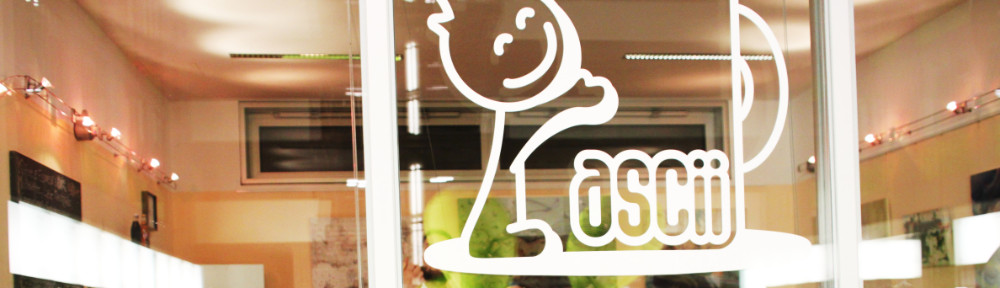
\includegraphics[width=\linewidth]{img/ascii.jpg}
\end{figure}

Das \ascii{} wird von einem studentischen Verein betrieben und ist seit seiner Gründung eine zentrale Anlaufstelle an der Fakultät.
Hier treffen sich Studierende und Beschäftigte, um ihre Pausen zu verbringen, zu arbeiten oder einfach ihren Koffeinhaushalt aufzufüllen.
Auf den gemütlichen Sofas kann man die Zeit wunderbar an sich vorbeistreichen lassen, gemeinsam an Projekten arbeiten, lernen, programmieren oder einfach nur mit Kommilitonen plaudern.

Wenn du jetzt Lust bekommen hast, das \ascii{} zu besuchen oder sogar als Mitglied selbst mitzumachen, dann komm doch einfach mal vorbei und sag Hallo!

Weitere Hinweise findest du unter~\link{https://www.ascii-dresden.de/}.

\begin{awesomeblock}[ese_bg_color]{2pt}{\faCalendar*[regular]}{ese_bg_color}
    \textbf{Öffnungszeiten während der Vorlesungszeit}

    Montag bis Donnerstag: 9 bis 17 Uhr

    Freitags: 9 bis 15 Uhr
\end{awesomeblock}
